\documentclass[tikz,border=0pt]{standalone}
\usepackage[T1]{fontenc}
\usepackage{lmodern}
\usepackage{xcolor}
\usepackage{amssymb}
\usetikzlibrary{arrows.meta,calc,fit,positioning,shapes.geometric,shapes.misc}

\definecolor{bg}{HTML}{F7F9FB}
\definecolor{ink}{HTML}{0B2239}
\definecolor{muted}{HTML}{41566B}
\definecolor{blue}{HTML}{0D4B7A}
\definecolor{lineblue}{HTML}{66B6FF}
\definecolor{cyan}{HTML}{21D6D6}
\definecolor{green}{HTML}{49D46B}
\definecolor{amber}{HTML}{F4B64D}
\definecolor{orange}{HTML}{F07A24}
\definecolor{coral}{HTML}{FF5A5F}
\definecolor{pink}{HTML}{FF6FAE}
\definecolor{violet}{HTML}{9B6CFF}
\definecolor{panel}{HTML}{F7F9FB}
\definecolor{soft}{HTML}{EEF4F8}
\definecolor{grayimg}{HTML}{D9DDE0}
\definecolor{graydark}{HTML}{38404A}

\tikzset{
  every node/.style={font=\sffamily, text=ink},
  panelbox/.style={
    draw=#1,
    fill=panel,
    fill opacity=0,
    text opacity=1,
    rounded corners=4pt,
    line width=.8pt,
    inner sep=6pt
  },
  card/.style={
    draw=#1,
    fill=bg,
    fill opacity=0,
    text opacity=1,
    rounded corners=4pt,
    line width=.8pt,
    align=center,
    inner sep=5pt
  },
  dashedbox/.style={
    draw=#1,
    fill=bg,
    fill opacity=0,
    text opacity=1,
    rounded corners=7pt,
    line width=1pt,
    dash pattern=on 4pt off 3pt,
    inner sep=7pt
  },
  flow/.style={
    -{Latex[length=2.6mm,width=1.9mm]},
    line width=.85pt,
    draw=#1
  },
  dotflow/.style={
    -{Latex[length=2.4mm,width=1.7mm]},
    line width=.8pt,
    draw=#1,
    dotted
  },
  title/.style={font=\sffamily\bfseries\Large, text=ink, align=left},
  subtitle/.style={font=\sffamily\bfseries\small, text=muted, align=left},
  small/.style={font=\sffamily\scriptsize, text=muted, align=center},
  tiny/.style={font=\sffamily\tiny, text=muted, align=center}
}

\newcommand{\panelbadge}[3]{%
  \node[circle, fill=blue, draw=lineblue, line width=.7pt, minimum size=.86cm,
    font=\sffamily\bfseries\Large, text=white] at (#1,#2) {#3};%
}

\newcommand{\microthumb}[3]{%
  \begin{scope}[shift={(#1,#2)}, scale=#3]
    \draw[fill=grayimg, draw=ink!35, line width=.35pt, rounded corners=.02cm] (0,0) rectangle (1.32,.82);
    \foreach \x/\y/\r in {.25/.42/.18,.52/.51/.14,.72/.33/.20,.93/.56/.13,.42/.22/.09,.98/.23/.08}
      \draw[fill=graydark!42, draw=graydark!78, opacity=.72] (\x,\y) circle (\r);
    \foreach \x/\y/\r in {.20/.63/.05,.68/.66/.04,1.12/.61/.06,1.12/.38/.05,.17/.18/.04}
      \draw[fill=white, draw=graydark, opacity=.55] (\x,\y) circle (\r);
    \draw[ink, line width=.08cm] (1.03,.08) -- (1.23,.08);
  \end{scope}
}

\newcommand{\segthumb}[3]{%
  \begin{scope}[shift={(#1,#2)}, scale=#3]
    \draw[fill=grayimg, draw=ink!35, line width=.35pt, rounded corners=.03cm] (0,0) rectangle (2.15,1.45);
    \foreach \x/\y/\r in {.38/.75/.25,.70/.92/.28,1.08/.78/.33,1.48/.84/.26,1.67/.45/.18,.55/.37/.16}
      \draw[fill=graydark!50, draw=graydark!85, opacity=.72] (\x,\y) circle (\r);
    \foreach \x/\y/\r/\c in {.35/.72/.20/cyan,.72/.89/.20/green,1.08/.77/.25/violet,1.44/.81/.20/orange,1.63/.47/.16/pink,.56/.38/.13/amber}
      \draw[fill=\c!55, draw=black, opacity=.72] (\x,\y) circle (\r);
  \end{scope}
}

\newcommand{\wrongmark}[2]{%
  \draw[coral, line width=1.8pt] (#1-.15,#2-.15) -- (#1+.15,#2+.15);
  \draw[coral, line width=1.8pt] (#1-.15,#2+.15) -- (#1+.15,#2-.15);
}

\newcommand{\dbicon}[3]{%
  \begin{scope}[shift={(#1,#2)}, scale=#3]
    \draw[fill=blue!70!black, draw=cyan, line width=.45pt] (0,0) ellipse (.42 and .13);
    \draw[fill=blue!35!black, draw=cyan, line width=.45pt] (-.42,0) -- (-.42,-.62)
      arc[start angle=180,end angle=360,x radius=.42,y radius=.13] -- (.42,0);
    \draw[draw=cyan!80, line width=.35pt] (-.42,-.31) arc[start angle=180,end angle=360,x radius=.42,y radius=.13];
  \end{scope}
}

\begin{document}
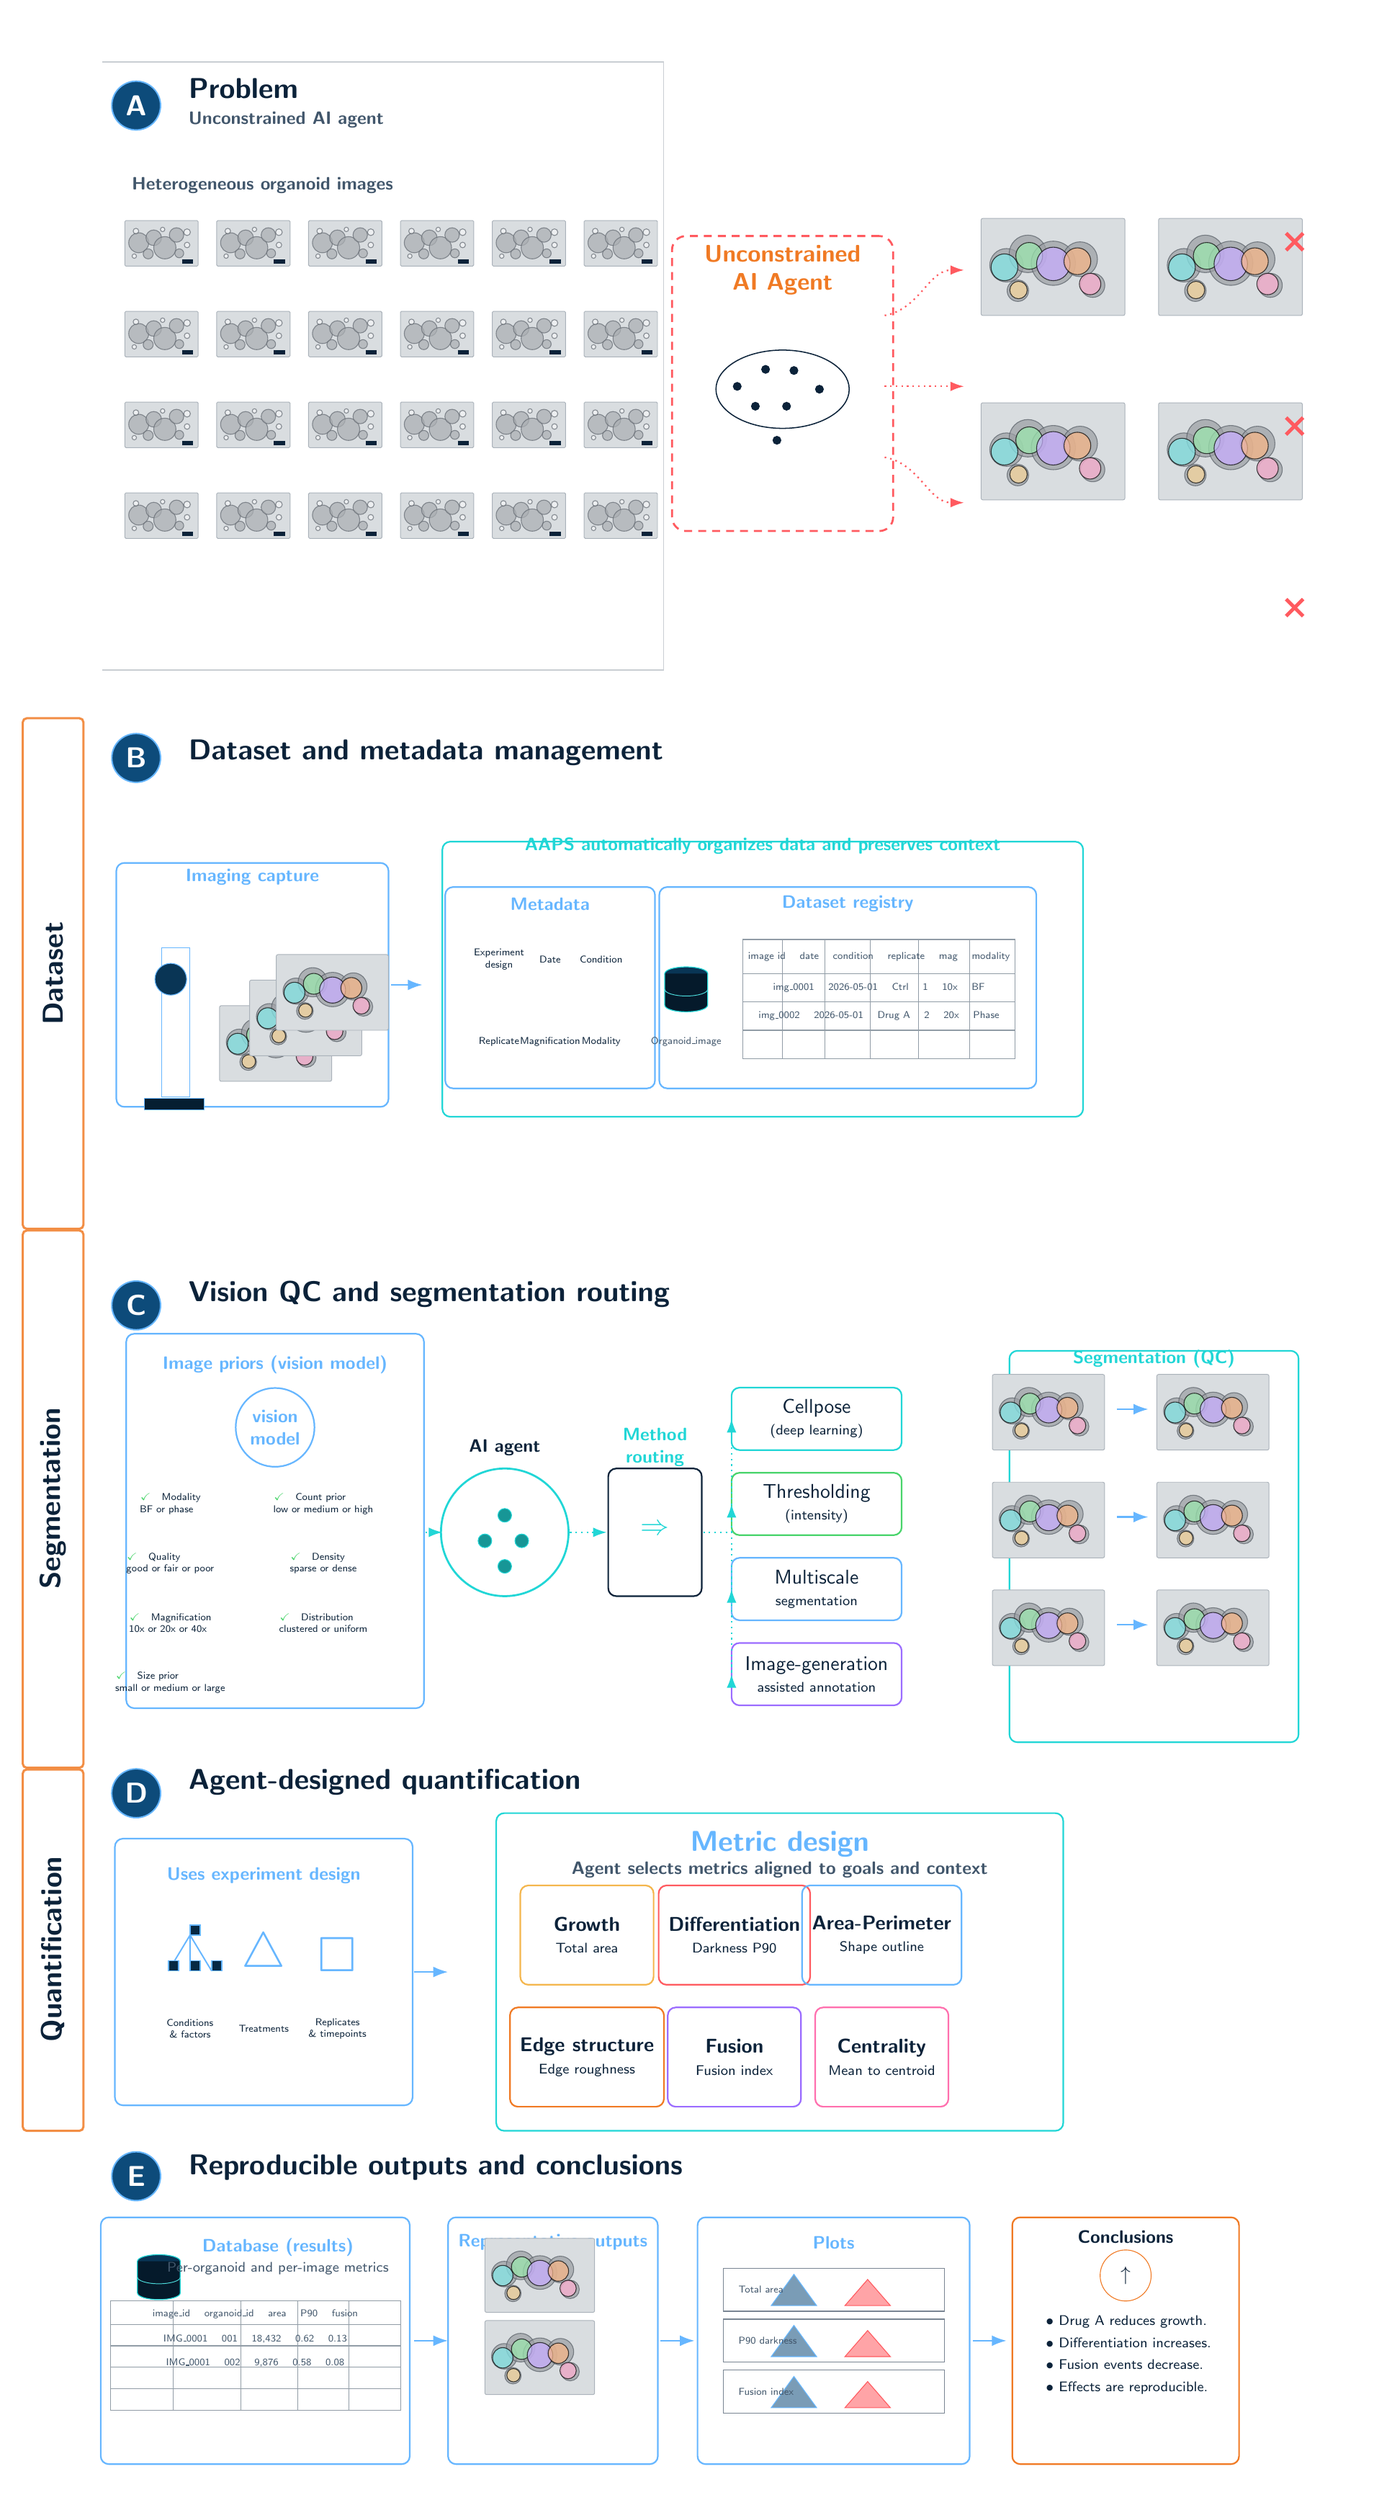
\begin{tikzpicture}[x=1cm,y=1cm]
  \path[use as bounding box] (0,0) rectangle (23.84,43.36);

  % Left structural bracket.
  \draw[orange!85, line width=1.1pt, rounded corners=2pt] (.05,22.05) rectangle (1.12,31.05);
  \draw[orange!85, line width=1.1pt, rounded corners=2pt] (.05,12.55) rectangle (1.12,22.02);
  \draw[orange!85, line width=1.1pt, rounded corners=2pt] (.05,6.15) rectangle (1.12,12.52);
  \node[font=\sffamily\bfseries\Large, text=ink, rotate=90] at (.58,26.55) {Dataset};
  \node[font=\sffamily\bfseries\Large, text=ink, rotate=90] at (.58,17.3) {Segmentation};
  \node[font=\sffamily\bfseries\Large, text=ink, rotate=90] at (.58,9.35) {Quantification};

  % Panel A.
  \panelbadge{2.05}{41.85}{A}
  \node[title, anchor=west] at (2.85,42.15) {Problem};
  \node[subtitle, anchor=west] at (2.85,41.6) {Unconstrained AI agent};
  \node[subtitle, anchor=west] at (1.85,40.45) {Heterogeneous organoid images};
  \draw[ink!22, line width=.55pt] (1.45,31.9) -- (11.35,31.9) -- (11.35,42.62) -- (1.45,42.62);
  \foreach \r in {0,...,3} {
    \foreach \c in {0,...,5} {
      \pgfmathsetmacro{\xx}{1.85+\c*1.62}
      \pgfmathsetmacro{\yy}{39.02-\r*1.6}
      \microthumb{\xx}{\yy}{.98}
    }
  }
  \node[dashedbox=coral, minimum width=3.9cm, minimum height=5.2cm] (badagent) at (13.45,36.95) {};
  \node[font=\sffamily\bfseries\large, text=orange, align=center] at (13.45,38.95) {Unconstrained\\AI Agent};
  \node[ellipse, draw=ink, line width=.55pt,
    minimum width=2.35cm, minimum height=1.38cm] at (13.45,36.85) {};
  \foreach \x/\y in {12.65/36.9,13.15/37.2,13.65/37.18,14.1/36.85,13.52/36.55,12.97/36.55,13.35/35.95}
    \node[circle, draw=ink, fill=ink, minimum size=.14cm, inner sep=0pt] at (\x,\y) {};
  \draw[dotflow=coral] (15.25,38.15) to[out=10,in=180] (16.65,38.95);
  \draw[dotflow=coral] (15.25,36.9) -- (16.65,36.9);
  \draw[dotflow=coral] (15.25,35.65) to[out=-10,in=180] (16.65,34.85);
  \segthumb{16.95}{38.15}{1.18}
  \segthumb{20.08}{38.15}{1.18}
  \segthumb{16.95}{34.9}{1.18}
  \segthumb{20.08}{34.9}{1.18}
  \wrongmark{22.48}{39.45}
  \wrongmark{22.48}{36.2}
  \wrongmark{22.48}{33.0}

  % Panel B.
  \panelbadge{2.05}{30.35}{B}
  \node[title, anchor=west] at (2.85,30.45) {Dataset and metadata management};
  \node[panelbox=lineblue, minimum width=4.8cm, minimum height=4.3cm] (capture) at (4.1,26.35) {};
  \node[subtitle, text=lineblue] at (4.1,28.25) {Imaging capture};
  \draw[fill=white!90, draw=lineblue] (2.5,24.38) rectangle (3.0,27.0);
  \draw[fill=blue!40!black, draw=lineblue] (2.2,24.15) rectangle (3.25,24.35);
  \draw[fill=blue!70!black, draw=lineblue] (2.66,26.45) circle (.28);
  \segthumb{3.52}{24.65}{.92}
  \segthumb{4.05}{25.1}{.92}
  \segthumb{4.52}{25.55}{.92}
  \draw[flow=lineblue] (6.55,26.35) -- (7.1,26.35);
  \node[panelbox=cyan, minimum width=11.3cm, minimum height=4.85cm] (registry) at (13.1,26.45) {};
  \node[font=\sffamily\bfseries\small, text=cyan] at (13.1,28.8)
    {AAPS automatically organizes data and preserves context};
  \node[card=lineblue, minimum width=3.7cm, minimum height=3.55cm] at (9.35,26.3) {};
  \node[subtitle, text=lineblue] at (9.35,27.78) {Metadata};
  \foreach \lab/\x/\y in {Experiment\\design/8.45/26.8,Date/9.35/26.8,Condition/10.25/26.8,Replicate/8.45/25.35,Magnification/9.35/25.35,Modality/10.25/25.35}
    \node[tiny, text=ink] at (\x,\y) {\lab};
  \node[card=lineblue, minimum width=6.65cm, minimum height=3.55cm] at (14.6,26.3) {};
  \node[subtitle, text=lineblue] at (14.6,27.78) {Dataset registry};
  \dbicon{11.75}{26.55}{.9}
  \node[tiny] at (11.75,25.35) {Organoid\_image};
  \draw[ink!45] (12.75,27.15) rectangle (17.55,25.05);
  \foreach \x in {13.45,14.2,15.0,15.85,16.75} \draw[ink!45] (\x,25.05)--(\x,27.15);
  \foreach \y in {25.55,26.05,26.55} \draw[ink!45] (12.75,\y)--(17.55,\y);
  \node[tiny] at (15.15,26.85) {image id \quad date \quad condition \quad replicate \quad mag \quad modality};
  \node[tiny] at (15.15,26.3) {img\_0001 \quad 2026-05-01 \quad Ctrl \quad 1 \quad 10x \quad BF};
  \node[tiny] at (15.15,25.8) {img\_0002 \quad 2026-05-01 \quad Drug A \quad 2 \quad 20x \quad Phase};

  % Panel C.
  \panelbadge{2.05}{20.7}{C}
  \node[title, anchor=west] at (2.85,20.9) {Vision QC and segmentation routing};
  \node[panelbox=lineblue, minimum width=5.25cm, minimum height=6.6cm] (priors) at (4.5,16.9) {};
  \node[subtitle, text=lineblue] at (4.5,19.65) {Image priors (vision model)};
  \node[circle, draw=lineblue, line width=.8pt, minimum size=1.1cm,
    font=\sffamily\bfseries\small, text=lineblue, align=center] at (4.5,18.55) {vision\\model};
  \node[tiny, align=left, text=ink] at (2.65,17.2) {\textcolor{green}{\(\checkmark\)}\quad Modality\\BF or phase};
  \node[tiny, align=left, text=ink] at (2.65,16.15) {\textcolor{green}{\(\checkmark\)}\quad Quality\\good or fair or poor};
  \node[tiny, align=left, text=ink] at (2.65,15.1) {\textcolor{green}{\(\checkmark\)}\quad Magnification\\10x or 20x or 40x};
  \node[tiny, align=left, text=ink] at (2.65,14.05) {\textcolor{green}{\(\checkmark\)}\quad Size prior\\small or medium or large};
  \node[tiny, align=left, text=ink] at (5.35,17.2) {\textcolor{green}{\(\checkmark\)}\quad Count prior\\low or medium or high};
  \node[tiny, align=left, text=ink] at (5.35,16.15) {\textcolor{green}{\(\checkmark\)}\quad Density\\sparse or dense};
  \node[tiny, align=left, text=ink] at (5.35,15.1) {\textcolor{green}{\(\checkmark\)}\quad Distribution\\clustered or uniform};
  \node[circle, draw=cyan, line width=1pt, minimum size=2.25cm] (cagent) at (8.55,16.7) {};
  \node[subtitle, text=ink] at (8.55,18.2) {AI agent};
  \foreach \x/\y in {8.2/16.55,8.85/16.55,8.55/17.0,8.55/16.1}
    \node[circle, fill=cyan!70!black, draw=cyan, minimum size=.24cm, inner sep=0pt] at (\x,\y) {};
  \draw[dotflow=cyan] (7.15,16.7) -- (7.45,16.7);
  \draw[dotflow=cyan] (9.7,16.7) -- (10.35,16.7);
  \node[card=ink, minimum width=1.65cm, minimum height=2.25cm] (route) at (11.2,16.7) {};
  \node[subtitle, text=cyan, align=center] at (11.2,18.2) {Method\\routing};
  \node[font=\Large, text=cyan] at (11.2,16.75) {$\Rightarrow$};
  \node[card=cyan, minimum width=3.0cm, minimum height=1.1cm] at (14.05,18.7) {Cellpose\\[-1pt]\scriptsize (deep learning)};
  \node[card=green, minimum width=3.0cm, minimum height=1.1cm] at (14.05,17.2) {Thresholding\\[-1pt]\scriptsize (intensity)};
  \node[card=lineblue, minimum width=3.0cm, minimum height=1.1cm] at (14.05,15.7) {Multiscale\\[-1pt]\scriptsize segmentation};
  \node[card=violet, minimum width=3.0cm, minimum height=1.1cm] at (14.05,14.2) {Image-generation\\[-1pt]\scriptsize assisted annotation};
  \foreach \yy in {18.7,17.2,15.7,14.2} \draw[dotflow=cyan] (12.05,16.7) -| (12.55,\yy) -- (12.55,\yy);
  \node[panelbox=cyan, minimum width=5.1cm, minimum height=6.9cm] at (20.0,16.45) {};
  \node[subtitle, text=cyan] at (20.0,19.75) {Segmentation (QC)};
  \foreach \r/\yy in {0/18.15,1/16.25,2/14.35} {
    \segthumb{17.15}{\yy}{.92}
    \draw[flow=lineblue] (19.35,\yy+.72) -- (19.9,\yy+.72);
    \segthumb{20.05}{\yy}{.92}
  }

  % Panel D.
  \panelbadge{2.05}{12.1}{D}
  \node[title, anchor=west] at (2.85,12.3) {Agent-designed quantification};
  \node[panelbox=lineblue, minimum width=5.25cm, minimum height=4.7cm] at (4.3,8.95) {};
  \node[subtitle, text=lineblue] at (4.3,10.65) {Uses experiment design};
  \begin{scope}[shift={(3.0,9.25)}]
    \draw[lineblue, line width=.7pt] (0,.35) -- (-.38,-.28) (0,.35) -- (0,-.28) (0,.35) -- (.38,-.28);
    \foreach \x/\y in {0/.35,-.38/-.28,0/-.28,.38/-.28}
      \draw[fill=blue!55!black, draw=lineblue, line width=.55pt] (\x,\y) rectangle ++(.18,.18);
  \end{scope}
  \node[font=\Huge, text=lineblue] at (4.3,9.25) {$\triangle$};
  \node[font=\Huge, text=lineblue] at (5.6,9.25) {$\square$};
  \node[tiny, text=ink] at (3.0,7.95) {Conditions\\\& factors};
  \node[tiny, text=ink] at (4.3,7.95) {Treatments};
  \node[tiny, text=ink] at (5.6,7.95) {Replicates\\\& timepoints};
  \draw[flow=lineblue] (6.95,8.95) -- (7.55,8.95);
  \node[panelbox=cyan, minimum width=10.0cm, minimum height=5.6cm] at (13.4,8.95) {};
  \node[font=\sffamily\bfseries\Large, text=lineblue] at (13.4,11.2) {Metric design};
  \node[subtitle, text=muted] at (13.4,10.75) {Agent selects metrics aligned to goals and context};
  \foreach \name/\sub/\x/\y/\col in {Growth/Total area/10.0/9.6/amber,Differentiation/Darkness P90/12.6/9.6/coral,Area-Perimeter/Shape outline/15.2/9.6/lineblue,Edge structure/Edge roughness/10.0/7.45/orange,Fusion/Fusion index/12.6/7.45/violet,Centrality/Mean to centroid/15.2/7.45/pink} {
    \node[card=\col, minimum width=2.35cm, minimum height=1.75cm] at (\x,\y) {\textbf{\name}\\[-1pt]\scriptsize \sub};
  }

  % Panel E.
  \panelbadge{2.05}{5.35}{E}
  \node[title, anchor=west] at (2.85,5.5) {Reproducible outputs and conclusions};
  \node[panelbox=lineblue, minimum width=5.45cm, minimum height=4.35cm] at (4.15,2.45) {};
  \dbicon{2.45}{3.85}{.9}
  \node[subtitle, text=lineblue] at (4.55,4.1) {Database (results)};
  \node[small] at (4.55,3.72) {Per-organoid and per-image metrics};
  \draw[ink!45] (1.6,3.15) rectangle (6.72,1.22);
  \foreach \x in {2.7,3.9,4.9,5.8} \draw[ink!45] (\x,1.22)--(\x,3.15);
  \foreach \y in {1.6,1.98,2.36,2.74} \draw[ink!45] (1.6,\y)--(6.72,\y);
  \node[tiny] at (4.15,2.92) {image\_id \quad organoid\_id \quad area \quad P90 \quad fusion};
  \node[tiny] at (4.15,2.48) {IMG\_0001 \quad 001 \quad 18,432 \quad 0.62 \quad 0.13};
  \node[tiny] at (4.15,2.06) {IMG\_0001 \quad 002 \quad 9,876 \quad 0.58 \quad 0.08};
  \draw[flow=lineblue] (6.95,2.45) -- (7.55,2.45);
  \node[panelbox=lineblue, minimum width=3.7cm, minimum height=4.35cm] at (9.4,2.45) {};
  \node[subtitle, text=lineblue] at (9.4,4.18) {Representative outputs};
  \segthumb{8.2}{2.95}{.9}
  \segthumb{8.2}{1.5}{.9}
  \draw[flow=lineblue] (11.3,2.45) -- (11.9,2.45);
  \node[panelbox=lineblue, minimum width=4.8cm, minimum height=4.35cm] at (14.35,2.45) {};
  \node[subtitle, text=lineblue] at (14.35,4.18) {Plots};
  \foreach \yy/\lab in {3.35/Total area,2.45/P90 darkness,1.55/Fusion index} {
    \draw[ink!55] (12.4,\yy-.38) rectangle (16.3,\yy+.38);
    \draw[lineblue, fill=blue!55] (13.25,\yy-.28) -- (13.65,\yy+.27) -- (14.05,\yy-.28) -- cycle;
    \draw[coral, fill=coral!55] (14.55,\yy-.28) -- (14.95,\yy+.18) -- (15.35,\yy-.28) -- cycle;
    \node[tiny, anchor=west] at (12.55,\yy) {\lab};
  }
  \draw[flow=lineblue] (16.8,2.45) -- (17.4,2.45);
  \node[panelbox=orange, minimum width=4.0cm, minimum height=4.35cm] at (19.5,2.45) {};
  \node[subtitle, text=ink] at (19.5,4.28) {Conclusions};
  \node[circle, draw=orange, minimum size=.9cm] at (19.5,3.6) {\(\uparrow\)};
  \node[small, align=left, text=ink] at (19.55,2.2) {\(\bullet\) Drug A reduces growth.\\[3pt]\(\bullet\) Differentiation increases.\\[3pt]\(\bullet\) Fusion events decrease.\\[3pt]\(\bullet\) Effects are reproducible.};
\end{tikzpicture}
\end{document}
